\documentclass[journal]{IEEEtran}
\usepackage{cite}
\usepackage{amsmath,amssymb,amsfonts,amsthm}
\usepackage{graphicx}
\usepackage{booktabs}
\usepackage{xcolor}
\usepackage{tikz}
\usetikzlibrary{positioning,arrows.meta}
\usepackage[hidelinks]{hyperref}
\newtheorem{proposition}{Proposition}

\begin{document}

\title{MIZAN: Balancing DDoS Mitigation and Service Outages with Safety-Spanning Group-Relative Policy Optimisation}

\author{Author~One, Author~Two, and Author~Three%
\thanks{The authors are with Affiliation, City, Country (e-mail: author1@institution.edu; author2@institution.edu; author3@institution.edu).}}

\markboth{IEEE Networking Letters}{MIZAN: Balancing DDoS Mitigation and Service Outages}

\maketitle

\begin{abstract}
Group Relative Policy Optimization (GRPO) can train 6G edge DDoS defenders without a critic or a learned attacker, but we show that it discards any safety cost shared by every rollout in a group. GRPO-trained defenders leak less traffic yet cause more severe outages than Sentinel, a co-evolutionary neuro-symbolic baseline. MIZAN adds one safe-side rollout per group, moved along a direction proven not to increase collateral damage, together with an outage budget. Over ten seeds, MIZAN beats Sentinel's checkpoints in all eight attack scenarios, cuts severe outages by 57\% and meets the outage budget in nine seeds.
\end{abstract}

\begin{IEEEkeywords}
DDoS mitigation, 6G security, safe reinforcement learning, group-relative policy optimisation.
\end{IEEEkeywords}

% ===========================================================================
\section{Introduction}
% ===========================================================================
\IEEEPARstart{Z}{ero-touch} 6G management expects edge controllers to absorb volumetric DDoS floods in closed loop~\cite{benzaid2020zsm,liyanage2023oran}. Such a controller must discard hostile traffic without starving legitimate users: a filter that is too aggressive causes the outage it was meant to prevent~\cite{guo2020xai6g}. Deep reinforcement learning has been applied to throttling, SDN flow control and per-host drop policies~\cite{malialis2015distributed,liu2018drlddos,simpson2020perhost}. Sentinel~\cite{alfatemi2026sentinel} is the most complete recent design. It trains its agent with Proximal Policy Optimization (PPO)~\cite{schulman2017ppo} against a co-evolving attacker and inserts a symbolic shield~\cite{alshiekh2018shielding} between the agent and the network. Its authors report that training deteriorates late in every seed and that severe outages persist under heavy floods.

Group Relative Policy Optimization (GRPO)~\cite{shao2024deepseekmath} looks like a natural successor. It compares several rollouts started from one state, so neither a value network nor a learned opponent is needed. In a simulator these rollouts can share one realisation of the traffic process~\cite{ng2000pegasus}, so that they differ only in the defender's actions. We find, however, that GRPO defenders leak less attack traffic than Sentinel but cause \emph{more} severe outages. The reason is structural. A cost that every member of a group incurs is removed by the group mean, mirroring the gradient starvation of binary-reward GRPO~\cite{nie2026starvation,yu2025dapo}. Separate normalisation of the cost channel, as in Constrained GRPO~\cite{girgis2026cgrpo}, does not help when that channel has no variance within a group. Injecting reference samples into groups stabilises language-model training~\cite{yan2025luffy,armor2026}, but no safe direction is available in that setting.

This letter makes three contributions. First, it formalises this \emph{constraint-cancellation} effect and confirms it on 80 trained checkpoints. Second, it proposes MIZAN (Arabic for \emph{balance}), whose \emph{safe-side member} keeps every group straddling the outage boundary, with a monotonicity guarantee. Third, it compares MIZAN with Sentinel's released checkpoints, a compute-matched PPO baseline, Constrained GRPO and the simplest alternative remedies over ten seeds.

% ===========================================================================
\section{System Model}
% ===========================================================================
\begin{figure}[t]
\centering
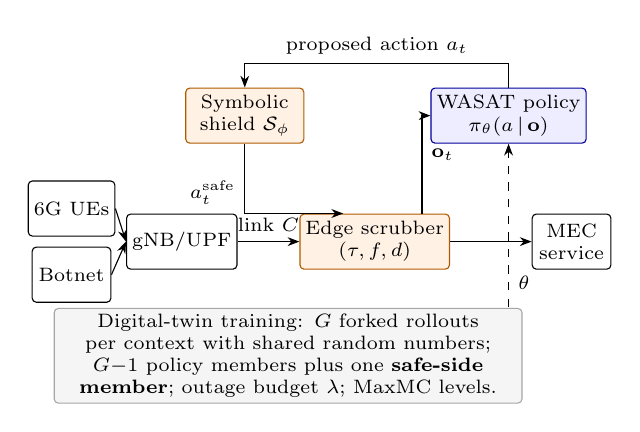
\begin{tikzpicture}[font=\scriptsize, >={Stealth[length=1.5mm]},
  box/.style={draw, rounded corners=1.5pt, align=center, inner sep=2pt, minimum height=7mm, fill=white},
  ag/.style={box, fill=blue!7, draw=blue!60!black}, sy/.style={box, fill=orange!10, draw=orange!70!black},
  tr/.style={box, fill=gray!8, draw=gray!70}]
\node[box, minimum width=10mm] (ue) at (0, 0.42) {6G UEs};
\node[box, minimum width=10mm] (bot) at (0,-0.42) {Botnet};
\node[box, minimum width=11mm] (gnb) at (1.4, 0) {gNB/UPF};
\node[sy, minimum width=17mm] (scr) at (3.85, 0) {Edge scrubber\\$(\tau,f,d)$};
\node[box, minimum width=10mm] (mec) at (6.35, 0) {MEC\\service};
\node[ag, minimum width=19mm] (pol) at (5.55, 1.6) {WASAT policy\\$\pi_\theta(a\,|\,\mathbf{o})$};
\node[sy, minimum width=15mm] (sh) at (2.2, 1.6) {Symbolic\\shield $\mathcal{S}_\phi$};
\node[tr, text width=58mm] (twin) at (2.75,-1.45) {Digital-twin training: $G$ forked rollouts per context with shared random numbers; $G{-}1$ policy members plus one \textbf{safe-side member}; outage budget $\lambda$; MaxMC levels.};
\draw[->] (ue.east) -- (gnb.west);
\draw[->] (bot.east) -- (gnb.west);
\draw[->] (gnb) -- node[above]{link $C$} (scr);
\draw[->] (scr) -- (mec);
\draw[->] ([xshift=6mm]scr.north) |- node[pos=0.3, right]{$\mathbf{o}_t$} (pol.west);
\draw[->] (pol.north) -- ++(0,0.3) -| node[pos=0.25, above]{proposed action $a_t$} (sh.north);
\draw[->] (sh.south) |- node[pos=0.35, left]{$a^{\mathrm{safe}}_t$} ([xshift=-4mm]scr.north);
\draw[->, dashed] (twin.east -| pol.south) ++(0,0.62) -- node[pos=0.15, right]{$\theta$} (pol.south);
\end{tikzpicture}
\caption{System model. At the 6G edge, a learned filtering policy configures a scrubber placed in front of the MEC service, and every proposal passes through a symbolic shield. The policy is trained in a digital twin using safety-spanning rollout groups.}
\label{fig:system}
\end{figure}

We use the setting of~\cite{alfatemi2026sentinel}, illustrated in Fig.~\ref{fig:system}. An edge link of capacity $C$ carries benign traffic $L_t\sim\mathrm{Poisson}(\mu)$ and attack traffic $A_t=1.5\,C\,i_t$. The attack belongs to a family in $\{\mathrm{SYN},\mathrm{UDP},\mathrm{HTTP},\mathrm{ICMP},\mathrm{mixed}\}$, with intensity $i_t\in[0,1]$ and a mutation level $m_t$ that weakens filter matching; flash crowds may inflate $L_t$ up to fourfold. ICMP is withheld from training. In each control window the defender observes twelve aggregate indicators $\mathbf{o}_t\in[0,1]^{12}$, measured on served traffic. It then sets a load threshold $\tau_t$, a filtering focus $f_t\in\{\mathrm{SrcIP},\mathrm{Proto},\mathrm{Size}\}$ and a drop probability $d_t$. With match effectiveness $\eta=\eta_{kf}(1-m_t/2)$, the share of benign traffic lost to filtering is
\begin{equation}
\mathrm{CD}_t = 0.4\,d_t(1-\eta)\,\alpha(\tau_t) + 0.2\,[L_t-C\tau_t]^+/L_t ,
\label{eq:cd}
\end{equation}
where $\alpha(\tau)$ is the fraction of offered load above the threshold. Service quality is $\mathrm{SQ}_t=\rho_t(1-\mathrm{CD}_t)$, with congestion factor $\rho_t=\min\{1,C/(L_t+A_t)\}$. A window with $\mathrm{SQ}_t<0.5$ is a \emph{severe outage}. The operator scores each window with Sentinel's benchmark,
$b_t=\mathrm{SQ}_t-\mathrm{leak}_t-0.5\,\mathbf{1}[\mathrm{SQ}_t<0.5]-0.25\,\mathbf{1}[\mathrm{SQ}_t<0.75]$,
where $\mathrm{leak}_t$ is the share of attack traffic delivered. A symbolic shield $\mathcal{S}_\phi$ edits unsafe actions through per-coordinate clamps. The defender solves
\begin{equation}
\max_\theta\ \mathbb{E}_{\pi_\theta}\Big[\textstyle\sum_t b_t\Big]\quad\text{s.t.}\quad \sigma(\pi_\theta)\le\kappa=0.05 ,
\label{eq:cpomdp}
\end{equation}
where $\sigma$ is the severe-outage frequency on the operator's validation scenarios. The budget $\kappa$ was fixed before the ten-seed experiments.

% ===========================================================================
\section{Constraint Cancellation}
\label{sec:mechanism}
% ===========================================================================
GRPO copies each training context into $G$ members that replay the same traffic. Member $g$ collects objective $O_g=\sum_h b_h$ and outage count $K_g$ over $H$ windows. With a Lagrange multiplier $\lambda$, the return is $R_g=O_g-\lambda K_g$ and the advantage is $\hat A_g=(R_g-\bar R)/s_R$, normalised by the group mean and standard deviation.

\begin{proposition}\label{prop:cancel}
If $K_g\equiv K$ within a group, then $\hat A_g$ is identical for all $\lambda\ge0$. The same holds for channel-wise normalisation $\hat A_g=\mathrm{z}(O)_g-\lambda\,\mathrm{z}(K)_g$~\cite{girgis2026cgrpo} with $\mathrm{z}(K)_g:=0$ when $s_K=0$.
\end{proposition}
\begin{proof}
$R_g-\bar R=O_g-\bar O$ and $s_R=s_O$; channel-wise, $s_K=0$ gives $\mathrm{z}(K)\equiv0$.
\end{proof}

The constraint therefore acts only through groups whose members disagree about the outage count; we call their share the \emph{span rate}. Leakage, being continuous, almost always varies. Under a full-intensity flood ($\rho_t\approx0.56$), a window becomes a severe outage once $\mathrm{CD}_t>1-0.5/\rho_t\approx0.10$. This threshold moves with the intensity, which is hard to observe once the link saturates. As GRPO sharpens its policy, whole groups fall beyond the threshold, and only the leakage term keeps steering the update.

Fig.~\ref{fig:mech} tests this explanation on 80 trained checkpoints under overload. The span rate grows with the within-group spread of the drop action ($r=0.91$), and checkpoints with a lower span rate suffer more severe outages ($r=-0.61$). Plain GRPO keeps a drop spread of 0.05, spans 47\% of groups and causes severe outages in 76\% of windows. PPO and Sentinel keep a spread above 0.21 and span every group.

\begin{figure}[t]
\centering
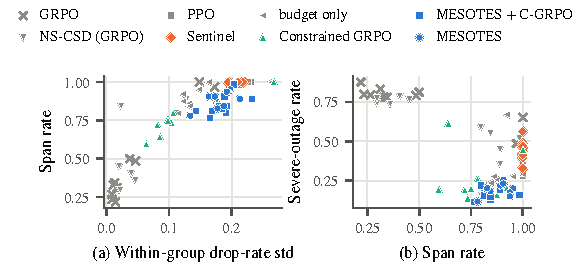
\includegraphics[width=\columnwidth]{figures/mechanism.pdf}
\caption{Constraint cancellation under full-intensity floods (80 checkpoints, $G=8$ members sharing traffic). (a) The span rate increases with the within-group spread of the drop action. (b) A lower span rate coincides with more severe outages.}
\label{fig:mech}
\end{figure}

% ===========================================================================
\section{MIZAN}
\label{sec:method}
% ===========================================================================
MIZAN reserves one \emph{safe-side member} per group. At each window it takes the policy's sample $(\tau,f,d)$, draws $u\sim\mathcal{U}(0.2,0.8)$ once per rollout, and executes $\tilde d=u\,d$, $\tilde\tau=\tau+(1-u)(1-\tau)$ and $\tilde f=f$.

\begin{proposition}\label{prop:safe}
For identical observations and traffic, the safe-side member's collateral damage after shielding never exceeds that of the policy member, so it never incurs more severe outages.
\end{proposition}
\begin{proof}
By~\eqref{eq:cd}, $\mathrm{CD}$ is non-decreasing in $d$ and non-increasing in $\tau$; $\eta$ is unchanged because $f$ is. Each shield rule is a per-coordinate $\min$ or $\max$ triggered by $(\mathbf{o}_t,f)$ only, so it preserves $\tilde d\le d$ and $\tilde\tau\ge\tau$. As $\rho_t$ does not depend on the action, $\mathrm{SQ}$ keeps the same order.
\end{proof}

Hence, whenever the sampled actions cause outages that a gentler filter would avoid, the safe-side member supplies the cost variance that Prop.~\ref{prop:cancel} shows to be necessary. The policy learns from it only through $-c\,[\hat A]^+\log\pi_\theta(\tilde a\,|\,\mathbf{o})$, that is, only when the member outperformed its group. The guarantee holds at every intensity, so MIZAN never needs to locate the threshold. Three further components complete the method:
\begin{itemize}
\item $\lambda$ follows dual ascent on the validation outage rate, $\lambda\leftarrow[\lambda+\eta_\lambda(\hat\sigma-\kappa)]^+$.
\item The deployed checkpoint is selected feasibility first.
\item Training contexts come from 360 discrete attack levels, prioritised by the MaxMC regret estimate~\cite{jiang2021robustplr,jiang2021plr} rather than by a learned attacker.
\end{itemize}
All GRPO variants share the remaining machinery: archive elites, shield probes, a KL anchor to the best validated checkpoint, and Sentinel's two-layer network trained without a critic.

% ===========================================================================
\section{Evaluation}
\label{sec:eval}
% ===========================================================================
We re-implemented Sentinel's public simulator and shield~\cite{sentinelcode} in batched form. Unit tests show agreement with the reference code to within $10^{-5}$, and Sentinel's released checkpoints reproduce its published strong-attack results (0.519/0.815/78.2 against 0.519/0.815/75.0 for quality, leakage and severe outages).

\textbf{Protocols.} We compare Sentinel's ten released checkpoints (seeds 42--51) with defenders trained on the same seeds. Protocol~B covers eight attack scenarios, four of them held-out stress tests, with 20 episodes of 100 windows each. Protocol~A replays the attacker that Sentinel trained for each seed, which is a transfer test for MIZAN. Protocol~C is a cross-entropy red team that searches the whole scenario space, ICMP included. All comparisons are paired by seed and traffic. We use paired $t$-tests with Holm correction and Wilcoxon tests.

\begin{table}[t]
\centering
\caption{Protocol B over 10 Seeds: Composite Score ($\uparrow$) and Severe Outages per 500 Windows ($\downarrow$)}
\label{tab:main}
\setlength{\tabcolsep}{2.4pt}
\resizebox{\columnwidth}{!}{%
\begin{tabular}{@{}lcccccc@{}}
\toprule
 & \multicolumn{3}{c}{Composite score} & \multicolumn{3}{c}{Severe outages} \\
\cmidrule(lr){2-4}\cmidrule(l){5-7}
Scenario & Sentinel & C-GRPO & IMBANG & Sentinel & C-GRPO & IMBANG \\
\midrule
Mild & 0.009 & \textbf{0.053} & 0.040\textsuperscript{\dag} & \textbf{0.0} & \textbf{0.0} & \textbf{0.0} \\
Strong & -0.746 & -0.612 & \textbf{-0.583}\textsuperscript{\dag} & 155.2 & 85.9 & \textbf{38.9} \\
Chaos/flash & -0.169 & \textbf{-0.114} & -0.123\textsuperscript{\dag} & 14.1 & 16.8 & \textbf{10.7} \\
ICMP (zero-shot) & -0.474 & -0.474 & \textbf{-0.458}\textsuperscript{\dag} & \textbf{4.6} & 23.3 & 18.0 \\
Pulsing$^\ast$ & -0.303 & -0.228 & \textbf{-0.225}\textsuperscript{\dag} & 60.5 & 37.7 & \textbf{16.1} \\
Polymorphic$^\ast$ & -0.454 & -0.442 & \textbf{-0.430}\textsuperscript{\dag} & 14.9 & 24.0 & \textbf{14.2} \\
Boundary$^\ast$ & 0.003 & \textbf{0.084} & 0.071\textsuperscript{\dag} & \textbf{0.0} & \textbf{0.0} & \textbf{0.0} \\
ICMP-chaos$^\ast$ & -0.299 & \textbf{-0.255} & -0.257\textsuperscript{\dag} & 25.4 & 25.2 & \textbf{20.9} \\
\midrule
Average & -0.304 & -0.248 & -0.246 & 34.4 & 26.6 & 14.8 \\
\bottomrule
\end{tabular}}

\vspace{2pt}
\parbox{\columnwidth}{\scriptsize $^\ast$Held-out stress test. \dag\,IMBANG above Sentinel, paired $t$-test, Holm-corrected, $p<0.05$. Bold: best.}
\end{table}


\textbf{Against Sentinel.} MIZAN scores significantly higher than Sentinel in every attack scenario (Table~\ref{tab:main}). The scenario average is $-0.246$ against $-0.304$ ($p=1.2\times10^{-5}$). Severe outages fall from 34.4 to 14.8 per 500 windows ($p=0.002$) and leakage from 0.876 to 0.839 ($p<10^{-3}$), with service quality unchanged. Against Sentinel's own attackers (Protocol~A), MIZAN also scores higher ($-0.265$ against $-0.332$, $p=0.019$). Its red-team worst case improves from $-1.07$ to $-0.72$ ($p=7.2\times10^{-4}$).

\textbf{Budget and remedies.} A PPO baseline given the same 1.34M training windows already improves on Sentinel, which shows the benefit of dropping co-evolution. MIZAN still beats it at equal budget ($+0.030$, $p=2\times10^{-7}$). Table~\ref{tab:ablation} and Fig.~\ref{fig:tradeoff} isolate the safe-side member:
\begin{itemize}
\item A Lagrangian budget alone is met in one seed out of ten even though $\lambda$ rises to about 7.7, as Prop.~\ref{prop:cancel} predicts.
\item An entropy bonus or an uncentred cost does not restore feasibility.
\item Constrained GRPO meets the budget in three seeds.
\item MIZAN meets it in nine with $\lambda\approx0.4$, matching Constrained GRPO's score ($p=0.47$) with fewer outages (14.8 against 26.6) and slightly more leakage (0.839 against 0.820).
\end{itemize}

\begin{table}[t]
\centering
\caption{Ablation and Alternative Remedies (10 Seeds). Worst: Red-Team Worst Case; Budget: Seeds Meeting $\sigma\le0.05$}
\label{tab:ablation}
\setlength{\tabcolsep}{3pt}
\resizebox{\columnwidth}{!}{%
\begin{tabular}{@{}lcccc@{}}
\toprule
Method & Score $\uparrow$ & Severe $\downarrow$ & Worst $\uparrow$ & Budget \\
\midrule
Sentinel~\cite{alfatemi2026sentinel} & -0.304 & 34.4 & -1.07 & -- \\
PPO + shield (equal budget) & -0.276 & 19.6 & -0.79 & -- \\
GRPO, no budget & -0.250 & 91.5 & -1.07 & -- \\
GRPO + budget & -0.253 & 36.5 & -0.87 & 1/10 \\
\;\; + entropy bonus $\times6$ & -0.249 & 33.8 & -0.85 & 0/10 \\
\;\; + uncentred cost & -0.251 & 34.7 & -0.87 & 1/10 \\
C-GRPO~\cite{girgis2026cgrpo} & -0.248 & 26.6 & -0.80 & 3/10 \\
\textbf{MIZAN} & -0.246 & 14.8 & -0.72 & 9/10 \\
MIZAN + C-GRPO normalisation & -0.247 & 12.1 & -0.71 & 7/10 \\
\bottomrule
\end{tabular}}
\end{table}


\begin{figure}[t]
\centering
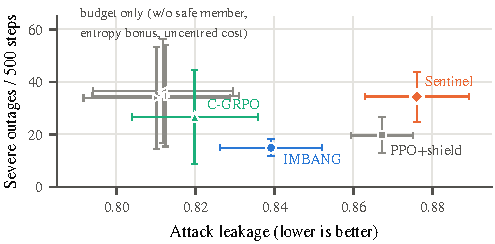
\includegraphics[width=\columnwidth]{figures/tradeoff.pdf}
\caption{Severe outages against attack leakage (Protocol~B, eight scenarios, 95\% confidence intervals over ten seeds). Only MIZAN reduces both relative to Sentinel.}
\label{fig:tradeoff}
\end{figure}

\textbf{Deployment and limitations.} The deployed actor has 5{,}447 parameters (21.8\,kB). On one 2.1\,GHz core, a decision including shielding takes 0.24\,ms, far below sub-second control windows. The study has four limitations:
\begin{itemize}
\item On zero-shot ICMP floods, MIZAN incurs more severe outages than Sentinel (18.0 against 4.6, not significant). A simulated operator playbook that reuses Sentinel's ICMP constants removes this gap.
\item MIZAN does not surpass Constrained GRPO on the composite score.
\item Prop.~\ref{prop:safe} assumes that congestion is evaluated on the offered load.
\item All results come from simulation.
\end{itemize}

% ===========================================================================
\section{Conclusion}
% ===========================================================================
Critic-free group-relative training removes the value network and the adversarial loop from DDoS defence, but it erases any safety cost that a whole group shares. A single safe-side member per group, guaranteed by monotonicity, restores that cost. The resulting defender outperforms the co-evolutionary Sentinel and more than halves its severe outages. Validation on replayed real traffic is left for future work.

\bibliographystyle{IEEEtran}
\bibliography{refs}

\end{document}
